\section{Introduction}
% \subsection{Motivation}

\begin{figure*}[tb!]
\begin{center}
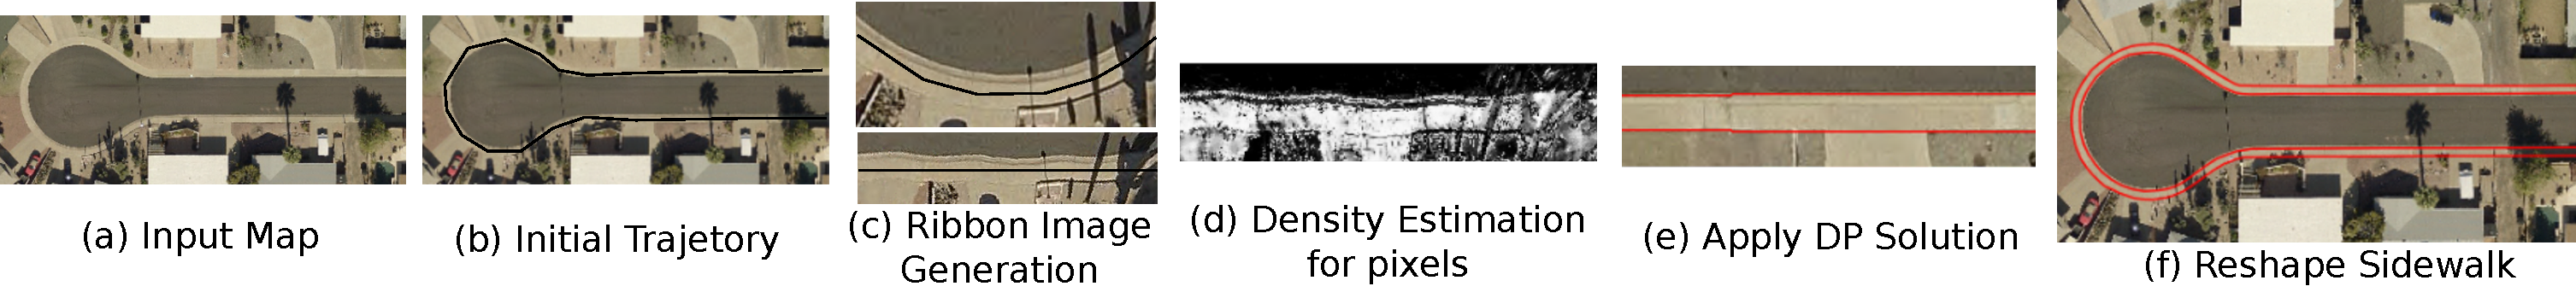
\includegraphics[width=\textwidth]{Figures/diagram.pdf}
\caption[Framework Overview]{Our approach to predict precise boundaries for ribbon-like features: black lines indicates the initial trajectory, and red lines show our predicted sidewalk boundaries.}
\label{fig:Apparatus}
\end{center}
\end{figure*}


Aerial imagery is an important resource for applications that include urban planning and map-making. 
Linear features such as sidewalks, street networks, canals, or biking paths are especially important because they provide essential connections between sites to support transportation of people and materials.
High-resolution aerial imagery has become a way to capture the appearance of these structures in order to look for changes such as new construction, damage, or obstructions. 

A \textit{ribbon-like} feature is a linear feature with varying thickness.
The scope of this paper is automatic refinement of previously digitized ribbon-like features, specifically walking paths, based on \ac{VHR} aerial imagery.
Given an approximate trajectory for the midline, and a range of potential thicknesses, we automate the process of estimating the most likely thicknesses and  trajectory of a path. 
One example of a downstream application would be an automatic method for precise localization and assessment of the quality of these pathways from geometric referenced imagery. 

Public domain or crowd-sourced repositories of spatial data such as \ac{OSM} \cite{OpenStreetMap} represent a very complete and frequently updated source of information which includes street vector data, and to a much lesser extent, the locations of foot-ways. 
However, the data is acquired from a variety of sources that may not be registered with enough precision to accurately place ribbon-like features. 
For thin structures such as sidewalks that are visible in \ac{VHR} imagery, even small discrepancies 
between the digitized pathways and the imagery can be distracting when used to visualize an overlaid 
map.  
As new \ac{VHR} aerial imagery becomes available thin features such as walking paths are discernible with higher precision,  but ortho-rectification processes may not precisely align the imagery with previously digitized features. 
In addition, poorly registered walking paths could confound any algorithm that might hope to automatically locate features on the path including obstacles, damage, overgrowth, or stairways that could impact the walk-ability. 
Several authors \cite{femiani2009interval, femiani2007road} have worked on segmenting streets directly from aerial imagery; however sidewalks are much thinner than streets and are often partially occluded. 
More importantly, these methods are mainly concerned with the connectivity of the extracted pathways and not with identifying the precise boundaries.
Our approach could be used to refine or recover the thickness of street networks or other networks of ribbon-like features.

Several automatic approaches \cite{ActiveContou09, Rother2004-ou, Achanta2012-ah} for image segmentation are able to locate precise object boundaries, especially for ``blobby" or compact regions.  
The \ac{SLIC} algorithm for super-pixels \cite{Achanta2012-ah} uses compact evenly distributed homogeneous regions of an image as a pre-processing step, so that image segmentation can be accomplished by grouping super-pixels which  snap to natural boundaries in an image. 
Alternatively, super-pixels can initiate a region growing process \cite{Borovec2017-fz}. A very 
successful region growing process is snakes, or \ActiveContours{}, \cite{ActiveContou09}, which starts 
with an approximate  contour and evolves the boundary to om an initial shape to find precise 
boundaries by solving a \ac{CRF} problem. 
In addition, graph cuts are capable of global \ac{CRF} optimization in some situations, and iterative graph cuts are used by the \GrabCut{} algorithm to refine an initial segmentation \cite{Rother2004-ou}.
However in \figref{fig:Method_comparison}optimize an energy function that favors likely contour 
shapes. 
Both \ac{SLIC} and active contours start fr we show the segmentation results of these methods, and 
note that  they struggle to constrain their results to ribbon-like shapes with smooth thickness and 
mid-line.
These color or boundary smoothness methods fail to capture an important quality of ribbon-like features, which is the thickness at one point depends not only on its adjacent points but also its topologically distant points along the contour.

\begin{figure}[tb]
    \centering
    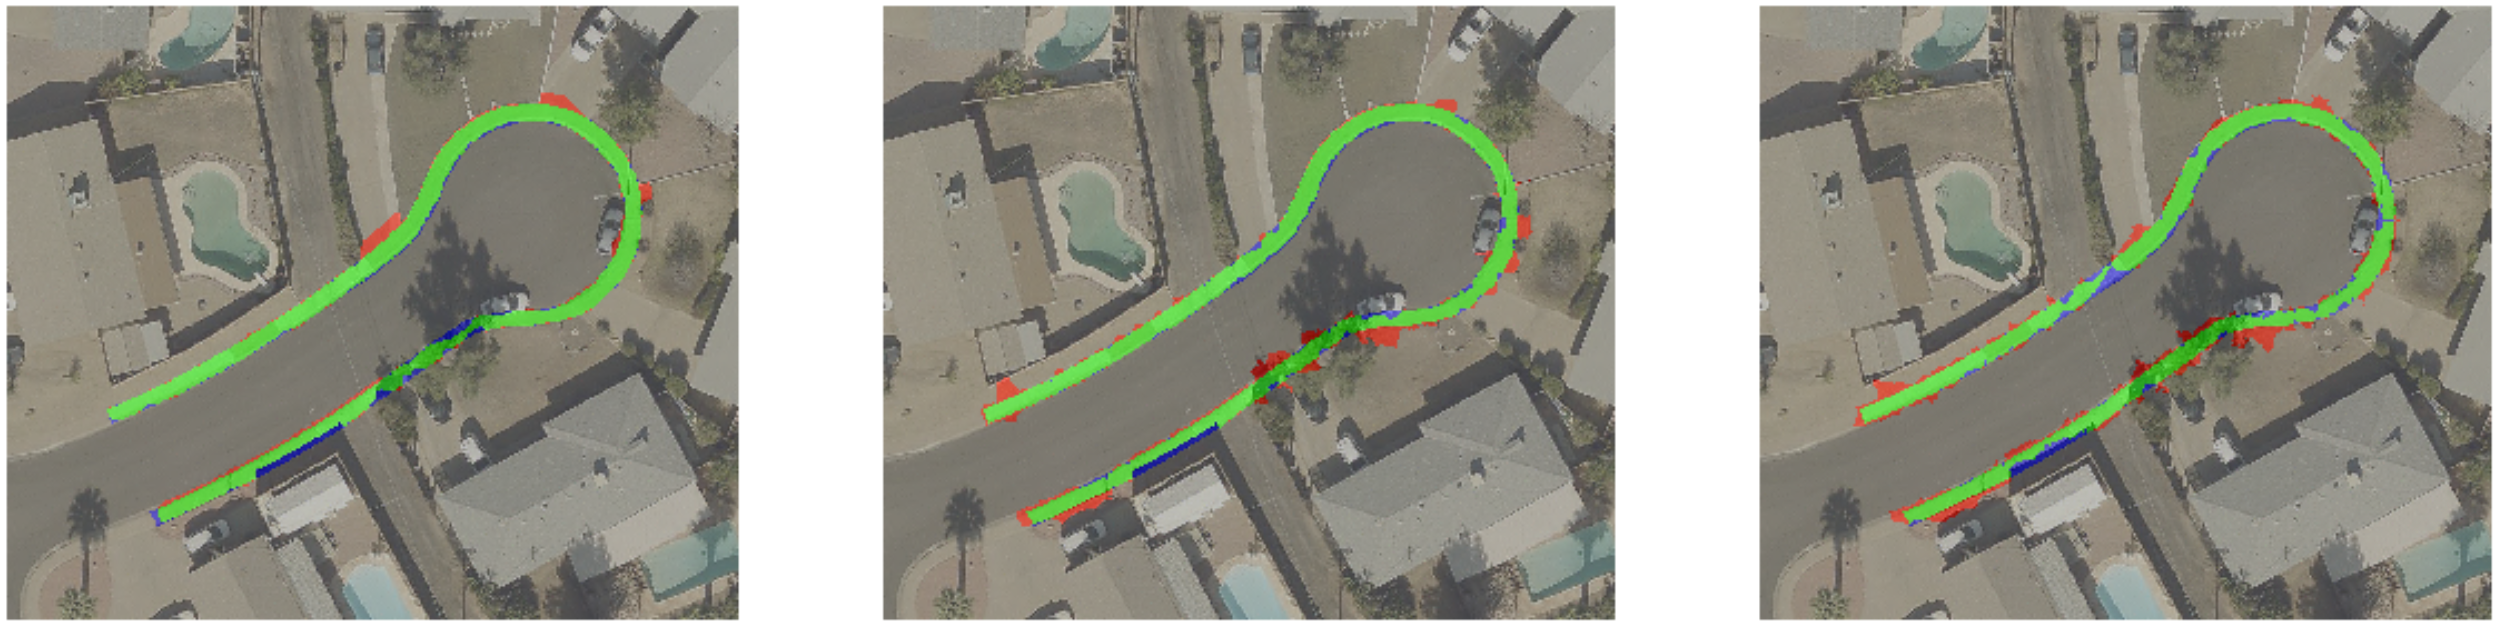
\includegraphics[width=0.95\columnwidth]{Figures/compare.png}
    \caption[Method comparison with \GrabCut{}, Active Contours, and \ac{SLIC}]{
        A comparison between\GrabCut{}(left), \ac{SLIC} (center) and \ActiveContours{} (right) 
        on an example of a sidewalk from 6-inch aerial imagery; 
        \aclp{TP} are rendered in green, 
        \aclp{FN} are rendered in blue, and 
        \aclp{FP} are rendered in red.  The \ac{SLIC} image contains all super-pixels that intersect the initial trajectory of a walking path; the \ActiveContours{} and \GrabCut{} methods are initialized with the \ac{SLIC} results.  
    }
    \label{fig:Method_comparison}
\end{figure}

% transposed convolutiuon == 'deconvolution'  -- the word deconvolution has another meaning in signal processing so we use transposed convolution instaed

% tunable is a word: https://www.merriam-webster.com/dictionary/tunable

%Another image segmentation approach that has seen extraordinary success is the
%use of \acp{CNN} and transposed convolution \cite{Ronneberger2015-sv,
%Shelhamer2017-rf, Noh2015-ni, Badrinarayanan2017-il}. Unlike the proposed
%approach, these have millions of tunable parameters and need significant
%pre-annotated data and offline training to build a model. In a recent
%exploration of learning to segment street networks from online maps,
%\cite{Kaiser2017-np} built a fully convolutional network with 137 million
%parameters. A similar approach with another deep architecture called U-net
%\cite{Ronneberger2015-sv} was applied to the street network segmentation
%problem \cite{Zhang2017-gi}. These approaches claim to be robust to occlusion
%and ambiguous regions, but they benefit from a large amount of carefully
%annotated data that includes road width \cite{Mnih2013-dp}. This type of
%pre-annotated data with aligned aerial imagery is much harder to obtain for
%walking paths.  The proposed approach has only a handful of tunable parameters
%with clear interpretations, so that they can be interactively set and used
%without offline training.

The main challenge addressed by our approach is to predict precise boundaries for ribbon-like walking paths when they are:
\begin{itemize}
    \item blocked by obstacles,
    \item under the shadow of trees, cars, or buildings,
    \item camouflage with adjacent materials (e.g. driveways, gutters),
    \item partially damaged so texture varies along the sidewalk.
\end{itemize}
Under these circumstances, most feature segmenting tools will not able to locate accurate boundaries. 

%To illustrate this challenge we look at the example of using \ac{SLIC} to
%segment the image in \figref{fig:slic}. In regions where shadows exist, the
%\ac{SLIC} superpixels snap to shadow boundaries instead of the target
%boundaries. 
%\begin{figure}
%    \centering
%    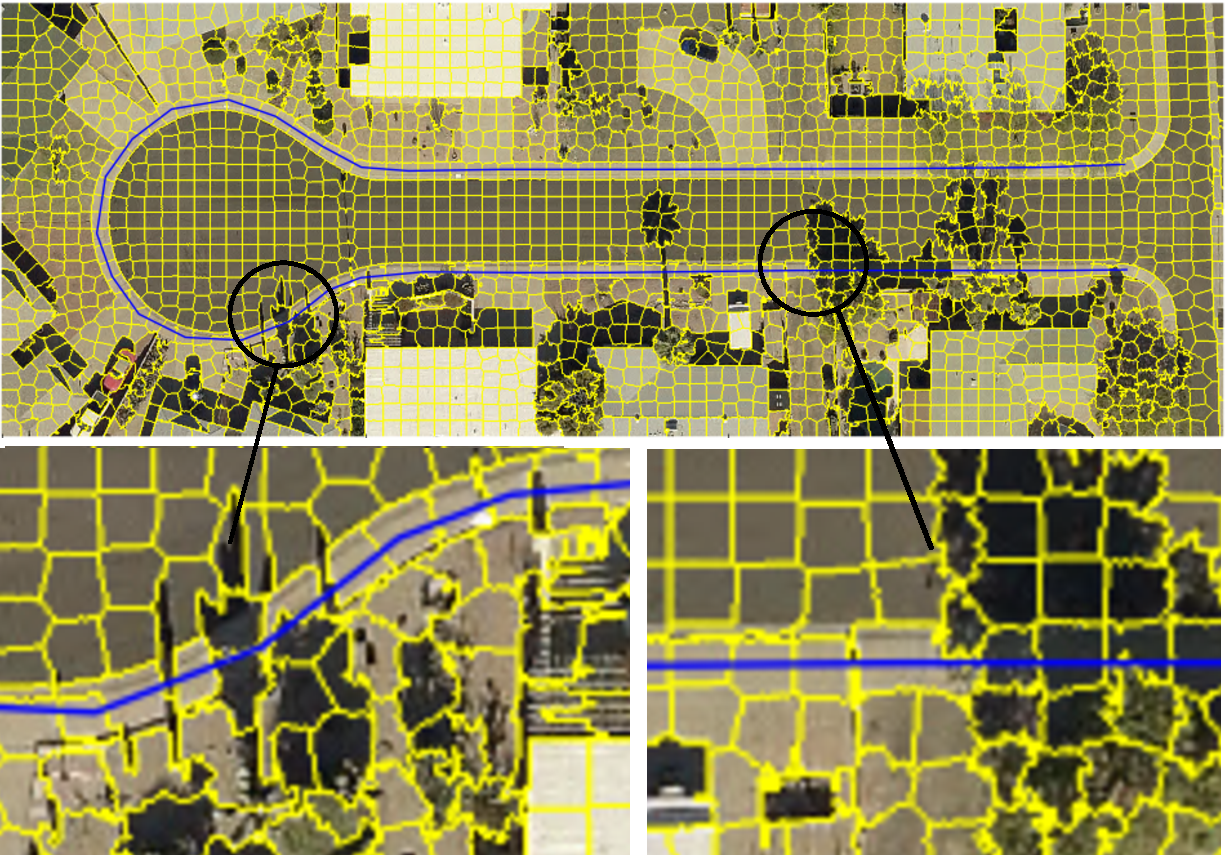
\includegraphics[width=0.95\columnwidth]{Figures/slic_sample1.pdf}
%    \caption[Example of Simple Linear Iterative Clustering]{Detail
%demonstration on segmenting large image into irregularly shaped super-pixels
%with \ac{SLIC}. Row 2 indicates examples of false positive, which recognized a
%non-sidewalk feature (shadow) as a part of sidewalk.}
%    \label{fig:slic}
%\end{figure}


\subsection{Contributions}
The aim of this work is to precisely align and determine the width of a coarsely registered ribbon-like feature to match its appearance in a \ac{VHR} image. 
The input is a \ac{VHR} georeferenced and orthorectified image along with a set of linear features that are close to, but perhaps not precisely aligned with the center of a ribbon-like feature. 
In particular, we expect that the ribbon will be made of a material with a somewhat uniform appearance (e.g. asphalt, gravel, or concrete) but that its appearance will be affected by shadows and interrupted by occlusions from vegetation, pedestrians, or vehicles such as bicycles.  
Our aim is to determine a more precise mid-line and an estimate for the width of the ribbon-like feature, which can vary slowly along its trajectory. 
The solution proposed in this paper does not rely on prior knowledge of the material on or around the ribbon, but instead, it estimates material appearance as it refines the placement of an initial estimate for the ribbon's mid-line.
	
Our contributions are as follows:
	\begin{itemize}
		\item A novel \ac{DP} approach is proposed for aligning ribbon-like features to orthoimagery.
		\item We do not require large training sets; a few parameters to control the smoothness of the resulting ribbon along with a coarse initial estimate of the trajectory are all that is needed. 
		\item Unlike methods that aim to recover the trajectories only, in our approach a likely thickness is directly identified so that more plausible trajectories and boundaries can be identified.
	\end{itemize}


\section{Approach} \label{sec:approach}

The main steps of our approach are illustrated in \figref{fig:Apparatus}; a \ac{VHR} orthorectified image is provided and the approximate trajectory of a sidewalk is acquired from a \ac{GIS} such as \ac{OSM}. Alternately, an approximate trajectory could be marked by a person to digitize the sidewalk quickly. The initial trajectory is re-sampled and used to warp a portion of aerial image so that the trajectory is mapped to a straight, horizontal line which we call a \textit{ribbon image}.  We use a modest assumption that colors near the center of the ribbon image are more likely to be on a walking path in order to build a probability-density estimate for walking path materials. Based on the probability estimate at each pixel, we construct a single ribbon with priors that control the rate of change of thickness and direction of the ribbon. Finally, the boundaries are warped back onto the original reference frame. In this section we elaborate the process of generating a ribbon image, estimating the probability that a color belongs to the same material as a walking path, and the construction of a smooth ribbon image based on the resulting probabilities. 



\subsection{Warping an input image}

We take as input an image $\InputImage{}$ and a trajectory $\InputTrajectory{}=\langle \vec{p}_0, \vec{p}_1,\dots,\vec{p}_m\rangle$ where each $\vec{p}_i=(x_i, y_i)^T$ is a point on the initial estimate of a ribbons trajectory (re-sampled to match the image resolution and smoothed). Further, we are able to estimate unit-length tangent vectors $\vec{u}_i$ and their perpendiculars $\vec{v}_i$; for example by using the secant method. 
%\begin{align}
%  \vec{u}_i &= \frac{\vec{p}_{i+1}-\vec{p}_{i-1}}{\|\vec{p}_{i+1}-\vec{p}_{i-1}\|} \\
%  \vec{v}_i &= \left(\begin{array}{cc}
%       0  & 1 \\
%       -1 & 0
%  \end{array} \right) \vec{u}_i
%\end{align}
%where the endpoints are repeated
We define the warped ribbon-image $\RibbonImage{}$ so that $\RibbonImage{[i,j]}=\InputImage{}(\vec{p}_i+ j \vec{v}_i)$. We use the convention that square-brackets to indicate discrete indices and rounded parenthesis indicate interpolated samples.  An example of the process is shown in \figref{fig:Sample_Sidewalk_4} and \figref{fig:Apparatus}(c). 

% \begin{figure}[ht]
%     \centering
%     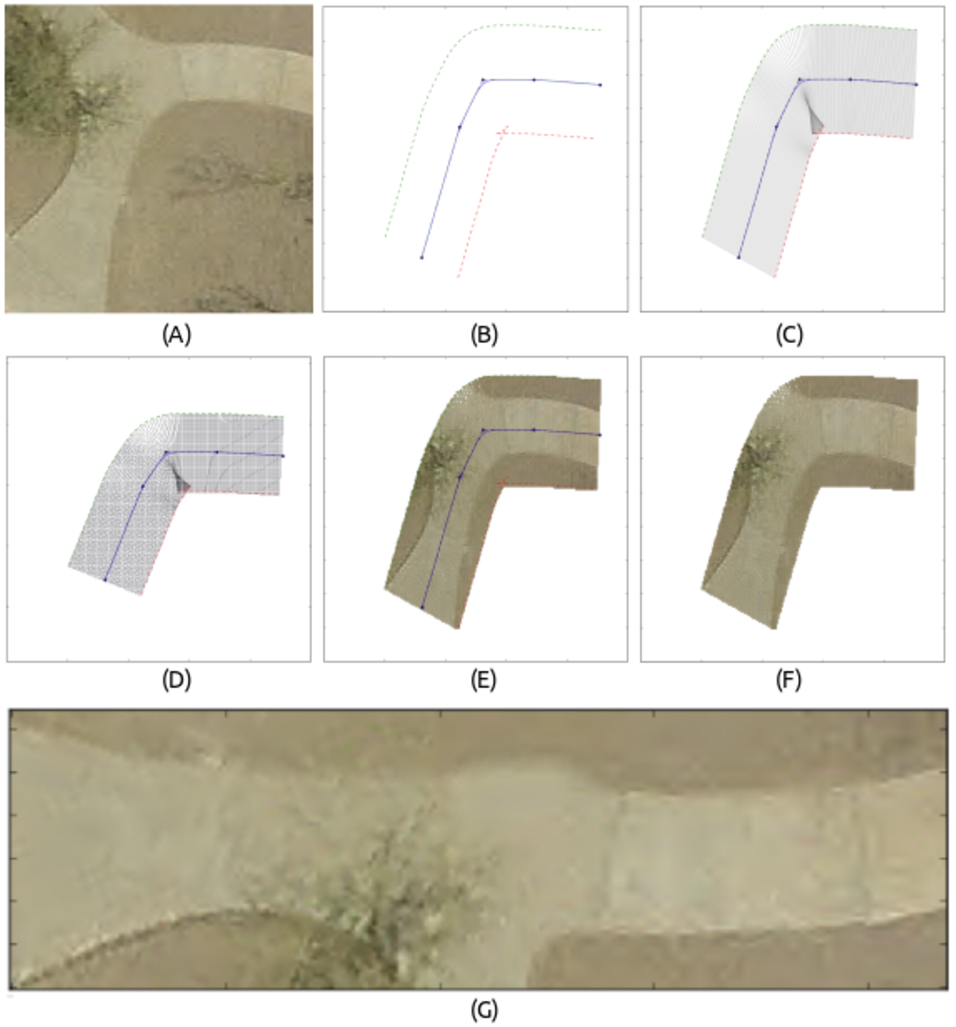
\includegraphics[width=0.95\columnwidth]{Figures/straghten.pdf}
%     \caption[Ribbon Image Generation]{Ribbon image generating process: (a) raw input $\InputImage{}$, (b) we densely resample and smooth the trajectory using $\MaxRadius{}$ iterations of Laplacian smoothing and show the locations of warped pixels of $\RibbonImage{}$ within $\pm \MaxDistance{}$;  (c) the warped ribbon image $\RibbonImage{}$ shown in the original reference frame and  (d) the generated the ribbon image (shown transposed to fit in the figure).}
%     \label{fig:StraightenProcess}
% \end{figure}

\begin{figure}[ht]
    \centering
    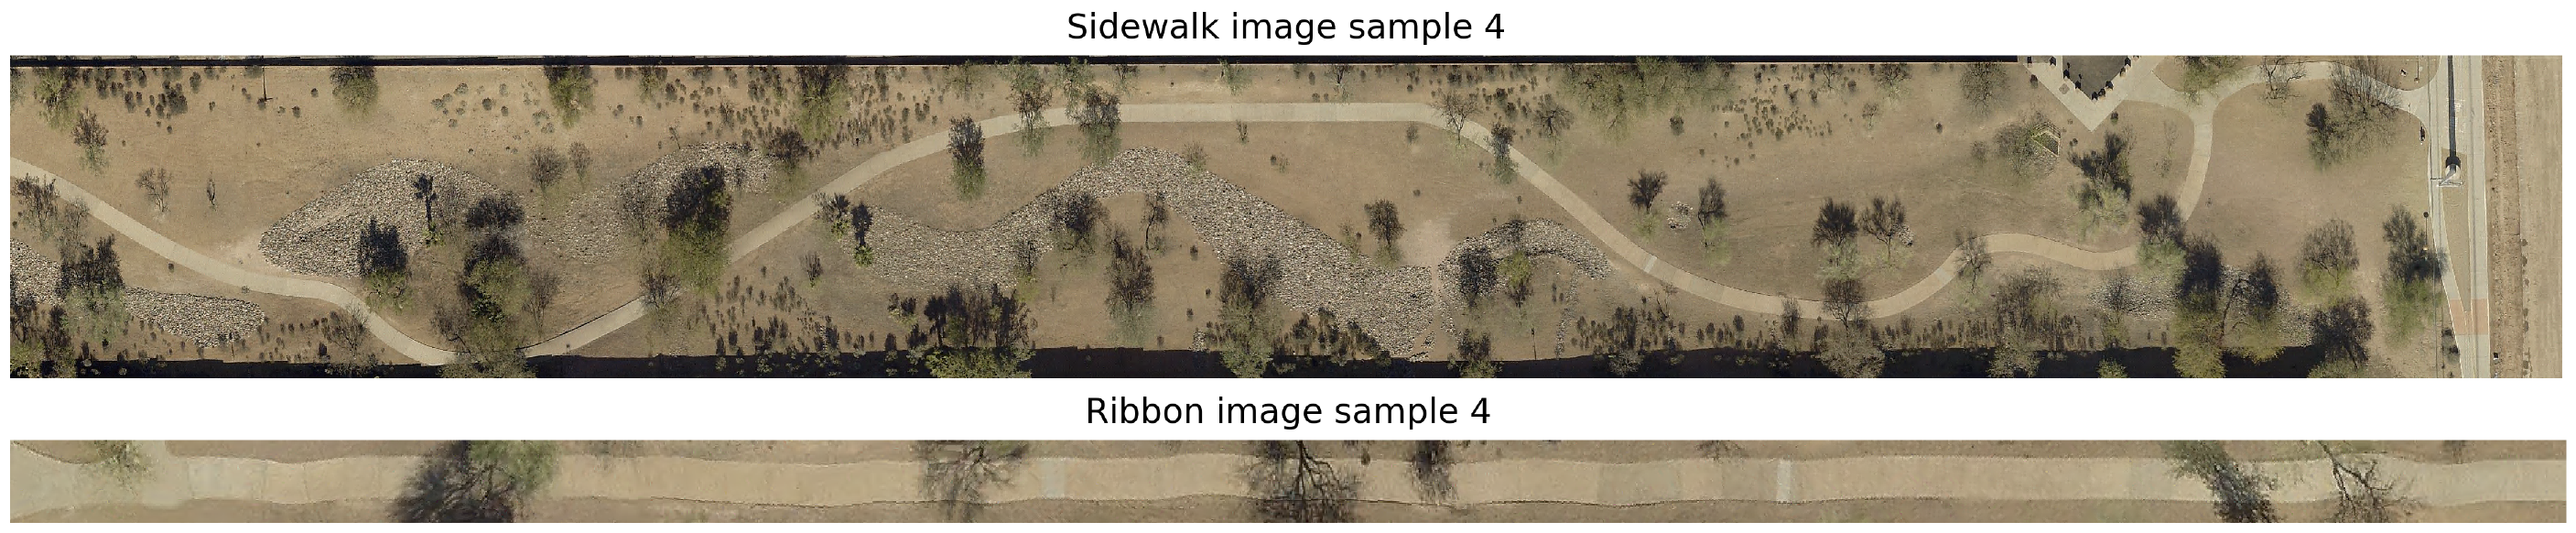
\includegraphics[width=0.95\columnwidth]{Figures/Sample4_needed.png}
    \caption[Sample Sidewalk]{A ribbon image; the original image $\InputImage{}$ (top) was warped so that the trajectory is a straight line to create a ribbon image $\RibbonImage{}$ (bottom), shown transposed.}
    \label{fig:Sample_Sidewalk_4}
\end{figure}

\subsection{Density Estimation}
We aim to find a new trajectory $\OutputTrajectory{[0\dots m]}$ and radius $\OutputRadius{[0\dots m]}$ that are most likely given an input image. We first must estimate the probability of observing a color within the ribbon.  
Given an input image $\RibbonImage{}$, let $\Pr(\text{pos}|\phi,\theta)$ denote the probability that a pixel is a part of a ribbon given an observed color $\phi$ and set of learnable parameters $\theta$. 
We aim to estimate parameters $\theta$ that maximize the likelihood of our \textit{initial} path. 
We do not in general have a reliable estimate for the initial radius of our ribbon, 
but we can construct a trimap (\figref{fig:ribbon_3d}, bottom), as is done by \GrabCut{}, in order to estimate $\theta$. We choose a distance $\MaxDistance$ and numbers $\MinRadius < \MaxRadius$ 
so that all pixels with a distance of $[0, \MinRadius)$ are likely part of the ribbon (positive), all pixels within a distance of $[\MinRadius, \MaxRadius)$ are unknown, and others are are assumed not to be part of the ribbon (negative); 
In our experiments we chose  $\MaxRadius$ as twice the expected mean width of ribbons (e.g. 2 meters), $\MinRadius = \MaxRadius/2$, and $\MaxDistance=\MaxRadius+\MinRadius$.  
In figure \ref{fig:ribbon_3d} these regions correspond to strips of pixels in $\RibbonImage{}$ along the edges and center of the image.

% \begin{figure}[h!]
%     \centering
%     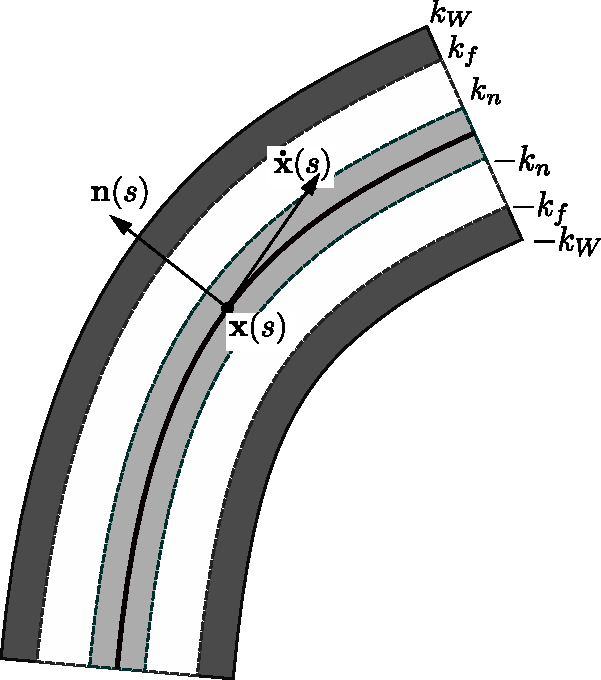
\includegraphics[width=0.3\textwidth]{Figures/sw-figure.pdf}
%     \caption[2D Ribbon Image]{A demonstration of the parameters for a ribbon in 2D, where $k_n$ indicates a lower-estimate for the radius of the ribbon, $k_f$ is an upper estimate, and $k_W$ is the maximum width of the ribbon image.}
%     \label{fig:2d_ribbon}
% \end{figure}

We use the \ac{EM-GMM} algorithm to find a max-likelihood estimate of $\theta$ as a pair of Gaussian mixtures so that $\Pr(\phi|\text{pos}, \theta)$ is a mixture of four multivariate Gaussian functions and $\Pr(\phi|\text{neg}, \theta)$ is a mixture of eight; then $\Pr(\text{pos}|\phi, \theta)$ can easily be found using Bayes theorem as 
$$\Pr(\text{pos}|\phi, \theta)= \frac{\Pr(\phi|\text{pos}, \theta)}{\Pr(\phi|\text{pos}, \theta)+\Pr(\phi|\text{neg}, \theta)}.$$


%\begin{figure}[htb]
%    \centering
%    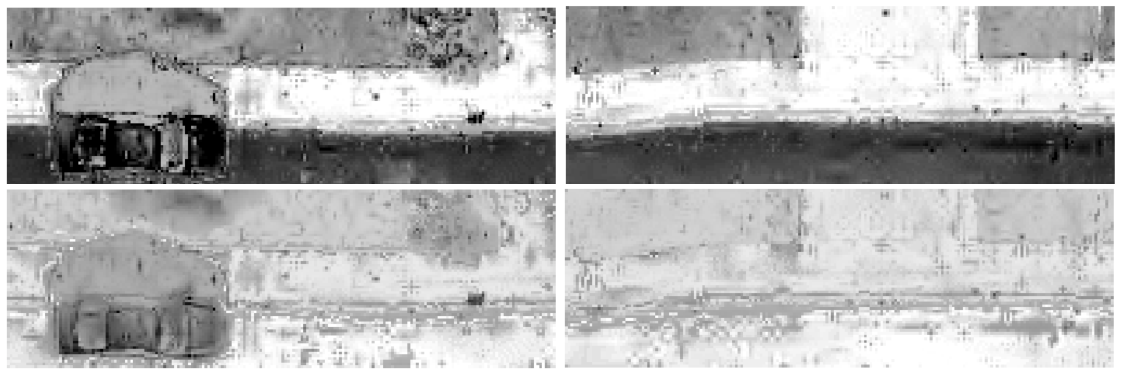
\includegraphics[width=0.95\columnwidth]{Figures/GMM_needed.pdf}
%    \caption[\ac{GMM} Result]{Example of probability density estimation for a sample sidewalk estimated as a pair of \acp{GMM} for positive (top) and negative (bottom) colors.}
%    \label{fig:GMM_result}
%\end{figure}

\FloatBarrier

The resulting probabilities are illustrated in
\figname{}~\ref{fig:Apparatus}(d); we observe that even a coarse initial
trajectory is usually enough to learn a more detailed, but noisy, estimate for
the foreground object shape. However colors alone are not able to discriminate
between occlusion and camouflage regions (such as the driveway in
\figname{}~\ref{fig:Apparatus}). For notational convenience we let
$p[i,j]=-\lg \Pr(\text{pos}|\RibbonImage{}[i,j], \theta)$ and 
$q[i,j]=-\lg \Pr(\text{neg}|\RibbonImage{}[i,j], \theta)$;
then the \ac{NLL} of a ribbon is proportional to a sum of $p[i,j]$ for all
$i,j$ within the ribbon and $q[i,j]$ for all $i,j$ outside the ribbon. The aim
of our \ac{DP} solution is to simultaneously optimize the probability based on
color and shape of a ribbon-like feature. 


\subsection{A Dynamic Programming Algorithm}

\begin{figure}[htb]
    \centering
    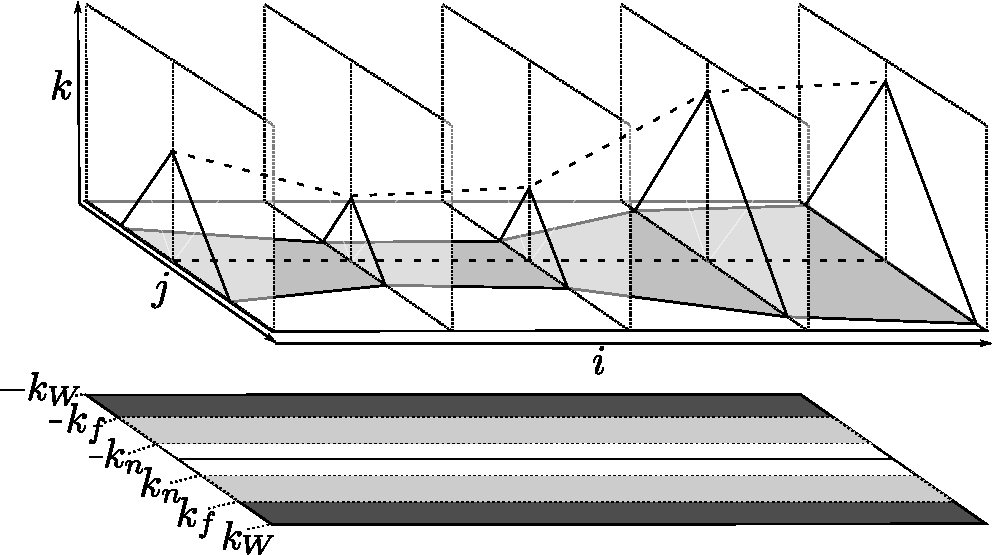
\includegraphics[width=0.95\columnwidth]{Figures/ribbon-3d-combined.pdf}
    \caption[3D Ribbon Image]{An illustration of the parameters for a ribbon: (top) the $k$ axis captures the thickness of the ribbon and the $i$ axis captures the distance along the initial ribbon, the $j$ axis records horizontal displacements from the initial ribbon's medial curve; (bottom) the boundaries of the ribbon must lie within $\pm \MaxDistance{}$, pixels within $\pm \MinRadius{}$ of the center are probably part of the ribbon and pixels further than $\pm \MaxRadius{}$ are likely negative. }
    \label{fig:ribbon_3d}
\end{figure}

We take $\RibbonImage{}$ as an input ribbon image with $m$ rows and $n=2\MaxDistance+1$ columns; $\RibbonImage{}{[i,j]}$ is a pixel in the image. We have an estimate $\Pr(\text{pos}|\RibbonImage{}_{[i,j]}, \theta)$ which we abbreviate as $p_{[i,j]})$. In addition there is some small set of allowed perturbations $\delta=\{(\delta_j, \delta_k)\}$ where $\delta_j$ is a change in direction and $\delta_k$ is a change in the radius of the ribbon. Each perturbation has a probability $\Pr(\delta_j, \delta_k)$ that controls the shape of the curve; in our experiments we use $\delta_j\in\{-1,0,1\}, \delta_k\in\{-1, 0,1\}$ in order to ensure that results are connected, and  $\Pr(\delta_j, \delta_k)=\Pr(|\delta_j|)\Pr(\delta_k)$ is two independent multinomial distributions which require only three parameters due to symmetry and because probabilities sum to unity. We can interpret $c_b=-\lg \Pr(\delta_j=\pm1)$ as a penalty for bending the curve, and $c_s=-\lg \Pr(\delta_k=-1)$ as a penalty for shrinking the radius, or $c_e = -\lg \Pr(\delta_k=1)$ as a penalty for expanding the radius of the curve. 

We visualize the problem of finding a ribbon as one of choosing a
three-dimensional path through a scale-space where the first two dimensions
represent locations of the ribbon's center, and the third dimension represents
the thickness of the ribbon as illustrated in \figref{fig:ribbon_3d}. Every
ribbon must start at one end of the image and follow a three-dimensional path
through scale-space to reach the other end one slice at a time. Each slice
corresponds to a row of the ribbon image and a point at location $(j, k)$ in the
slice partitions the row into negative regions $(0\twodots{}j-k-1)$ and
$(j+k+1\twodots{}n)$ with a positive region at $(j-k \twodots{} j+k)$ with
thickness $2k+1$. The likelihood of any location $(j, k)$ is the product of the
probabilities that each pixel on the same row belongs to the corresponding
positive or negative regions.  In fact the probability is exponentially related
to the size of each pixel; if one were to increase the resolution by a factor of
$r$ then the contribution of each pixel would be raised to the power of
$\frac{1}{r}$ so that the product would stay constant. In order to make our
parameters invariant to scale, we divide the \ac{NLL} by $\MaxDistance{}$ when
estimating the likelihood of a given $(j,k)$. 

We model the probability of a ribbon as the product of the probability of each location $(i, j, k)$ along the path times the probability of each edge from slice $i$ to slice $i+1$. We use dynamic programming to search to a path that minimizes the \ac{NLL} (the cost) of a path in procedure \proc{Segment-Ribbon}.

The pseudocode can be interpreted as follows: Line \ref{li:loop-slices} iterates through each slice of the ribbon image. Line \ref{li:loop-radius} iterates through all possible radii and line \ref{li:loop-center} explores all possible ribbon-centers from left to right. We use a variable $s$ to calculate the \ac{NLL} of a set of regions as the ribbon shifts from left to right. If this is not the first slice, then line \ref{li:min-from-pred} selects the least-expensive (most probable) path that leads to location $(i, j, k)$ in the scale space.  At each step one pixel toggles from negative to positive, and one toggles from positive to negative as $s$ is updated in line \ref{li:update-s}.  We return the costs as well as the final offset and scale $(j^*, k^*)$ of the best path. 


\begin{codebox}
\Procname{$\proc{Segment-Ribbon}(\RibbonImage{})$} \label{alg:segmet-ribbin}
\li $p[i,j]\gets -\lg \Pr(\RibbonImage{}[i,j])/\MaxDistance{}$, 
          \hspace{2ex} $q[i,j] \gets -\lg \Pr(1-\RibbonImage{}[i,j])/\MaxDistance{}$
\li $C{[0\twodots{}m, 0\twodots{}n, 0\twodots{}n]} \gets \infty$
\li \For{$i \gets 0 \To m$} \Do                                                \label{li:loop-slices}
\li     \For $k \gets 0 \To \lfloor n/2 \rfloor $ \Do                          \label{li:loop-radius}
\li         $s = \displaystyle{\sum_{j=0}^{2k} p[i,j] +\sum_{j=2k+1}^n  q[i, j] }$
\li         \For $j \gets k \To n-k$ \Do  \label{li:loop-center}
\li              \If $i > 0$  \Do                                              \label{li:if-has-pred}
\li              $v \gets s {+}\displaystyle{\min_{\delta_j, \delta_k}\left(  
                              \begin{aligned}
                              C[i{-}1,j{+}\delta_j,k{+}\delta_k] \hspace{3ex}\\
                              \hfill{}-\lg \Pr(\delta_j, \delta_k)
                              \end{aligned}
                            \right)}$  
                               \label{li:min-from-pred}
\li              \Else $v\gets s$
                 \End
\li              $C{[i, j, k]} \gets v$                                       \label{li:dp-store}
\li              $s \gets s{+}q[i,j{-}k]{-}p[i, j{-}k]{+}p[i, j{+}k]{-}q[i,j{+}k]$ \label{li:update-s}
           \End
       \End
    \End
\li $j^*, k^* \gets \displaystyle{\arg\min_{j,k} C{[m, j, k]}}$
\li \Return $C, j^*, k^*$
\end{codebox}

The \proc{Backtrack-Ribbon} algorithm selects the least-costly (most probable) ribbon and it is copied into to $T$ and $R$; so that the most likely path has scale-space coordinates $(i, T[i], R[i])$ for $i=0\twodots{}m$. 



\begin{codebox}
\Procname{$\proc{Backtrack-Ribbon}(C, j^*, k^*)$} \label{alg:backtrack-ribbon}
\li $T{[0{\twodots}m]} \gets 0$, \quad $R{[0{\twodots}m]} \gets 0$             
\li $T{[m]}, R{[m]} \gets j^*, k^*$ \label{li:backtrack-best-last}
\li \For $i \gets m-1 \Downto 0$ \Do
\li      $\delta_j, \delta_k = \displaystyle{\arg\min_{\delta_j,\delta_k}C{[i,j{-}\delta_j,k{-}\delta_l]}{-}\lg \Pr(\delta_j,\delta_k)}$
\li      $T{[i]}, R[i] \gets T{[i+1]}-\delta_j, R{[i+1]}-\delta_k$                                                 \label{li:backtack-choose-pred}
    \End
\li \Return $T, R, C_{[m, j^*, k^*]}$
\end{codebox}


If one wishes the path to be connected in scale-space, then there are only $3\times3$ possible values for $\delta_j, \delta_k$ in line \ref{li:min-from-pred}; so the algorithm is $\Theta(m n^2)$ and used $O(m n^2)$ space, where $m$ is the length of a ribbon and $n=2\MaxDistance+1$ is the maximum thickness of a ribbon. Since $\MaxDistance$ is typically a constant, this algorithm is effectively linear on the length of a ribbon. 



\section{Results}

We evaluate our results using precision ($P$), recall ($R$) and the balanced F-measure ($F_1$).
% defined as follows:
%\begin{align}
%     P &= \frac{\mathit{TP}}{\mathit{TP} + \mathit{FP}}, & 
%     R &= \frac{\mathit{TP}}{\mathit{TP} + \mathit{FN}}, &    
%     F_1 &= \frac{2 P R}{P + R}
%\end{align}
%where 
%\acp{TP} is the number of pixels correctly marked as positive, 
%\acp{FN} is the number incorrectly marked as negative and 
%\acp{FP} is the number incorrectly marked as positive. 

We compare our results against common segmentation approaches 
\ac{SLIC}~\cite{Achanta2012-ah}, \ActiveContours{}~\cite{ActiveContou09} and \GrabCut{}~\cite{Rother2004-ou} 
in Table~\ref{tab:quantitative-against-common} using a manually annotated region of 
Phoenix AZ. The test region was acquired as \ac{VHR} 4-inch aerial orthophotos, 
and manually annotated by drawing a polygonal outline. 
When a portion of the sidewalk was occluded or camouflage with the surrounding pavement 
(including gutters) we used our best judgment to connect the visible portions of the sidewalk. For all of of the examples we present, we set $c_\mathit{bend}=\frac{1}{2}, c_\mathit{shrink}=c_\mathit{expand}=2$ which were experimentally found to produce the best result. Note that in our implementation we did not take care to ensure that $\Pr(\delta_k)$ summed to unity, and instead assumed that $-\lg \Pr(\delta_k=0)$ was zero, which does not have a probabilistic interpretation but is more convenient for computation. 

\begin{table}[h!]
    \caption{Quantitative comparison. }
    \label{tab:quantitative-against-common}
    \centering
    \begin{tabular}{r ccc}
                            & $P$ & $R$& $F_1$ \\ 
                                 \hline 
                  \ac{SLIC} & 0.876 & 0.839 & 0.857 \\
          \ActiveContours{} & 0.873 & 0.866 & 0.869  \\
                 \GrabCut{} & 0.969 & 0.877 & 0.925  \\ 
                                 \hline
                \textbf{DP} & \textbf{0.973} & \textbf{0.961} & \textbf{0.967}   
    \end{tabular}
\end{table}

For qualitative comparison we compare against \ac{SLIC}, \ActiveContours{}, and \GrabCut{}, in \figref{fig:Sample_4_compare} and \figref{fig:Sample_2_compare}.  The former presents a portion of a hiking trail in a desert region where the foreground and background materials are similar and the path curves and varies in thickness. The \ac{DP} approach is smooth and also follows the boundary of the path closely, and it also follows a reasonable trajectory where the path bifurcates. More challenging scenarios are shown in \figref{fig:Sample_2_compare} which includes examples of occlusion, shadow, and camouflage.  

We have also identified the following limitations of the proposed method: it assumes that an initial ribbon overlaps with the feature in the corresponding orthophoto. We have not suggested an approach to determine if a walking path has been removed, or has been completely occluded. Furthermore, we assume \ac{VHR} orthoimagery that has enough resolution to build a model for colors on and off the ribbon. The proposed approach finds integer raddii, so thicknesses are all multiples of two. We recommend up-sampling images, which will allow the proposed approach to solve for a trajectory with sub-pixel precision. Finally, while we do make some assumptions when we select $\MinRadius{}, \MaxRadius{}, \MaxDistance{}$ the method as presented does not impose a prior on expected thickness of ribbons; often this is known and it could be used to generate plausible results for completely occluded ribbons. 

% \begin{figure}
%     \centering
%     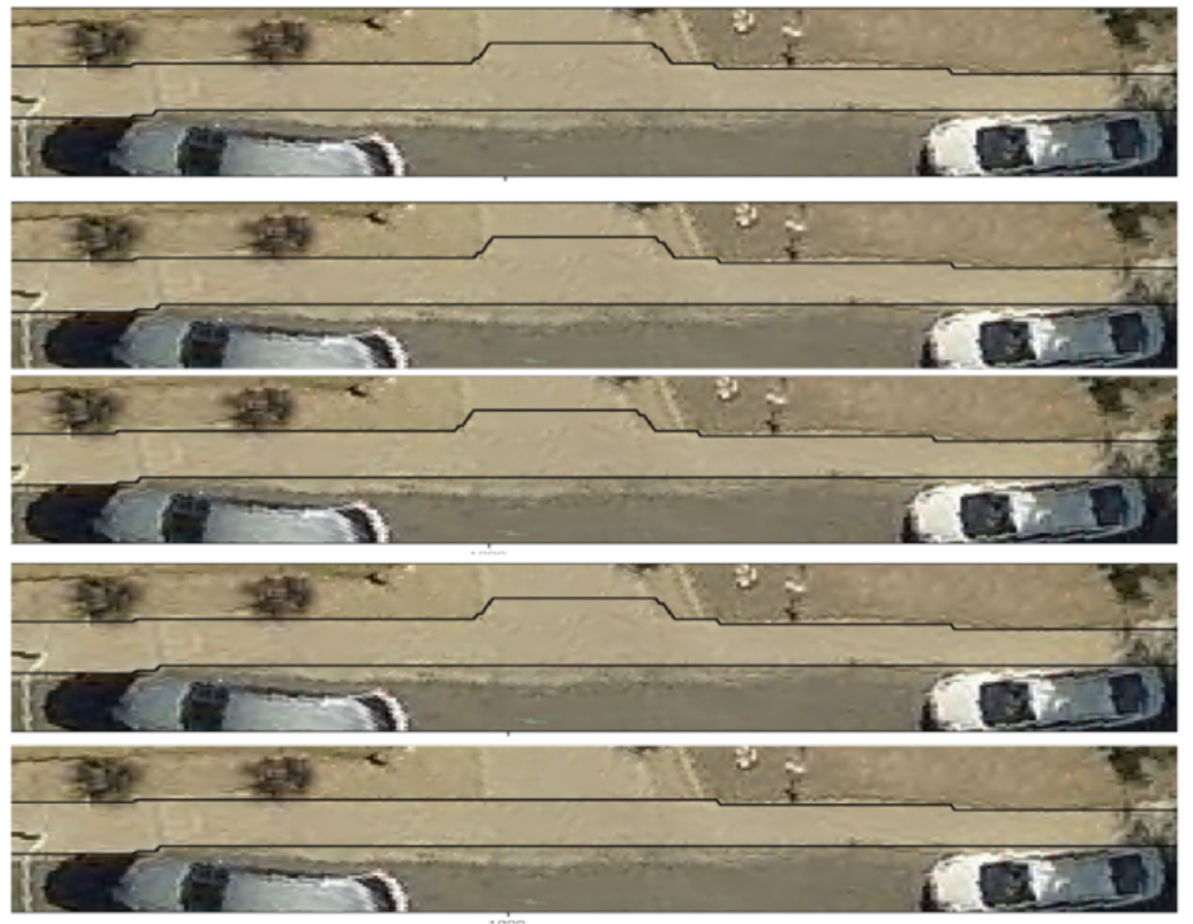
\includegraphics[width=0.95\columnwidth]{Figures/penalty.pdf}
%     \caption[Penalty Process]{Comparison with penalty change, we tested a variety of variables to decide which variable had best performance for width control. With the penalty increased at a reasonable amount, our algorithm decided not to recognize a driveway as sidewalk walk, in order to keep the sidewalk width consistent, even though they are the same texture.}
%     \label{fig:penalty}
% \end{figure}


\begin{figure}[htb]
    \centering
    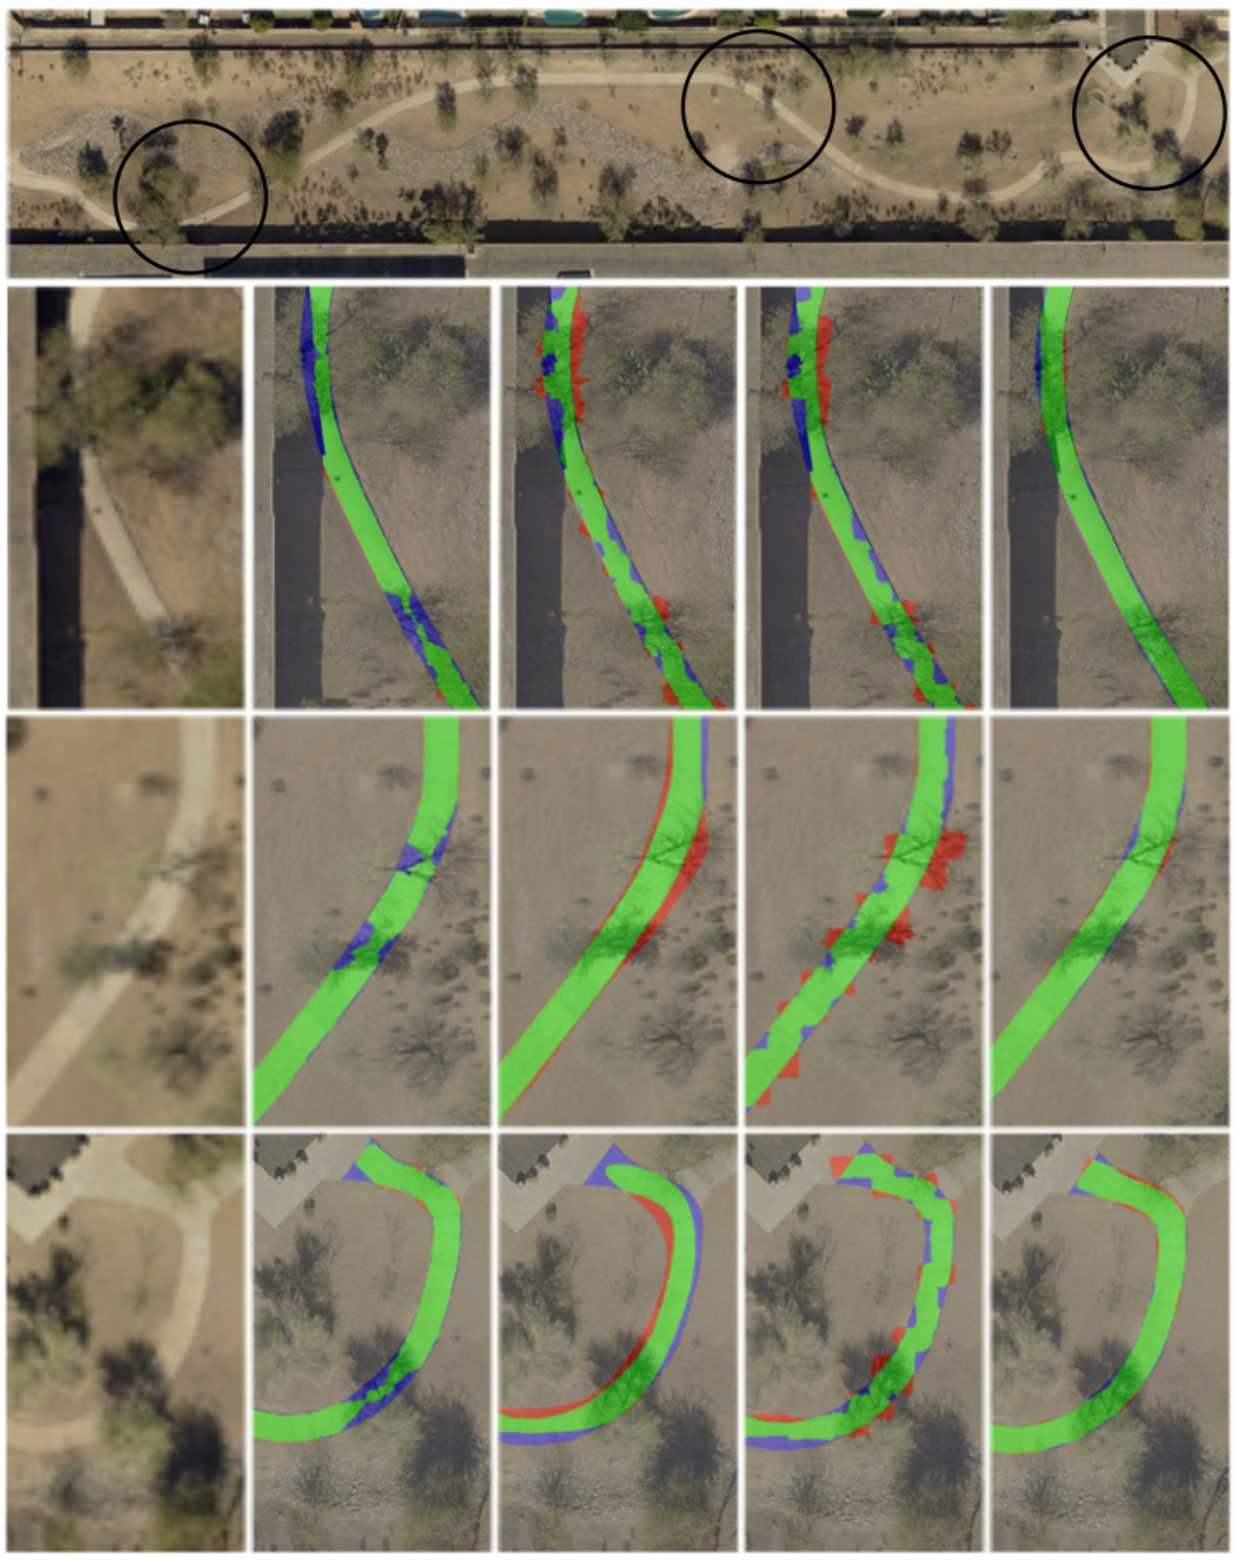
\includegraphics[width=0.95\columnwidth]{Figures/4_comparison.pdf}
    \caption[Methods Comparison on Sample Sidewalk]{A visual comparison between three different methods and ours \ac{DP} solution, from left to right we show the input, \GrabCut{}, \ac{SLIC}, \ActiveContours{} and our \ac{DP} result.}
    \label{fig:Sample_4_compare}
\end{figure}

\begin{figure}[htb]
    \centering
    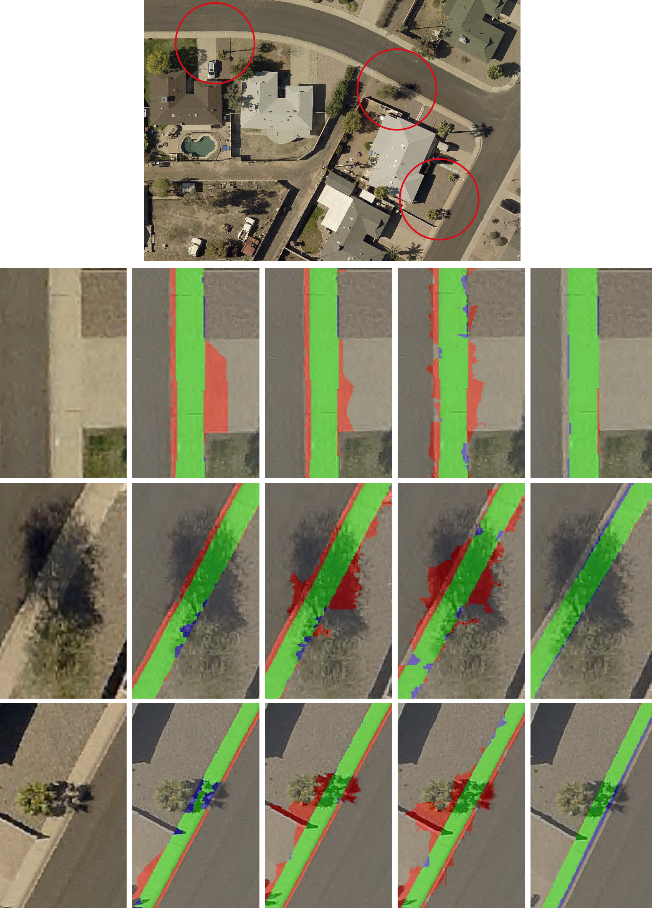
\includegraphics[width=0.95\columnwidth]{Figures/2_comparison_needed.png}
    \caption[Methods Comparison on More Sample Sidewalk]{A visual comparison between three different methods and ours \ac{DP} solution, from left to right we show the input, \GrabCut{}, \ac{SLIC}, \ActiveContours{} and our \ac{DP} result.}
    \label{fig:Sample_2_compare}
\end{figure}

\section{Conclusion}

A method to estimate the thickness and to refine the trajectory of a ribbon-like feature in \ac{VHR} aeral orthoimagery has been presented; we were able to obtain both high qualitative and quantitative results for segmenting walking paths in aerial imagery by refining \ac{OSM} features. The method is fast, and has only a few parameters with clear interpretations;
%we evaluate the effect of $c_\mathit{bend}$ to control the curvature of the ribbon's trajectory as well as $c_\mathit{shrink}$ and $c_\mathit{expand}$ to limit the variation in thickness.
The proposed approach does not rely on extensive training on annotated data, but instead learns to fit the underlying imagery based on a trimap that is specified by parameters $\MinRadius{}, \MaxRadius{}, \MaxDistance{}$ which values that are easily determined based on the task, and are unlikely to require adjustment. 

We evaluated this work by comparing it mainly to approaches for interactive image segmentation because most automatic approaches for extracting street-maps focus on extracting coarse trajectories (which we take as input) rather than on precise alignment and width estimation. We focused on modeling footways which are small, thin, easily occluded, and often modified due to construction. We believe that this approach is a natural tool to improve segmentation by post-processing automatically extracted street networks, and also by enabling fast interactive annotation of aerial images by refining hand-entered paths such as those found in \ac{OSM}.  


\FloatBarrier

% \begin{acks}
% % Thank anyone who provided data, code, or money, like who? 
% %  I will do it later. Acknowledgments will go in the final copy
% If you find anybody else to compare against and they gave us data (or results), we would acknowledge here

%   The authors would also like to thank the anonymous referees for
%   their valuable comments and helpful suggestions. The work is
%   supported by the Salt River Project (SRP) 

% \end{acks}
\